\documentclass[10pt, a5paper]{article}
\usepackage{pdfpages}
\usepackage{parallel}
\usepackage[T2A]{fontenc}
\usepackage{ucs}
\usepackage[utf8x]{inputenc}
\usepackage[polish,english,russian]{babel}
\usepackage{hyperref}
\usepackage{rotating}
\usepackage[inner=2cm,top=1.8cm,outer=2cm,bottom=2.3cm,nohead]{geometry}
\usepackage{listings}
\usepackage{graphicx}
\usepackage{wrapfig}
\usepackage{longtable}
\usepackage{indentfirst}
\usepackage{array}
\newcolumntype{P}[1]{>{\raggedright\arraybackslash}p{#1}}
\frenchspacing
\usepackage{fixltx2e} %text sub- and superscripts
\usepackage{icomma} % коскі ў матэматычным рэжыме
\PreloadUnicodePage{4}

\newcommand{\longpage}{\enlargethispage{\baselineskip}}
\newcommand{\shortpage}{\enlargethispage{-\baselineskip}}

\def\switchlang#1{\expandafter\csname switchlang#1\endcsname}
\def\switchlangbe{
\let\saverefname=\refname%
\def\refname{Літаратура}%
\def\figurename{Іл.}%
}
\def\switchlangen{
\let\saverefname=\refname%
\def\refname{References}%
\def\figurename{Fig.}%
}
\def\switchlangru{
\let\saverefname=\refname%
\let\savefigurename=\figurename%
\def\refname{Литература}%
\def\figurename{Рис.}%
}

\hyphenation{admi-ni-stra-tive}
\hyphenation{ex-pe-ri-ence}
\hyphenation{fle-xi-bi-li-ty}
\hyphenation{Py-thon}
\hyphenation{ma-the-ma-ti-cal}
\hyphenation{re-ported}
\hyphenation{imp-le-menta-tions}
\hyphenation{pro-vides}
\hyphenation{en-gi-neering}
\hyphenation{com-pa-ti-bi-li-ty}
\hyphenation{im-pos-sible}
\hyphenation{desk-top}
\hyphenation{elec-tro-nic}
\hyphenation{com-pa-ny}
\hyphenation{de-ve-lop-ment}
\hyphenation{de-ve-loping}
\hyphenation{de-ve-lop}
\hyphenation{da-ta-ba-se}
\hyphenation{plat-forms}
\hyphenation{or-ga-ni-za-tion}
\hyphenation{pro-gramming}
\hyphenation{in-stru-ments}
\hyphenation{Li-nux}
\hyphenation{sour-ce}
\hyphenation{en-vi-ron-ment}
\hyphenation{Te-le-pathy}
\hyphenation{Li-nux-ov-ka}
\hyphenation{Open-BSD}
\hyphenation{Free-BSD}
\hyphenation{men-ti-on-ed}
\hyphenation{app-li-ca-tion}

\def\progref!#1!{\texttt{#1}}
\renewcommand{\arraystretch}{2} %Іначай формулы ў матрыцы зліпаюцца з лініямі
\usepackage{array}

\def\interview #1 (#2), #3, #4, #5\par{

\section[#1, #3, #4]{#1 -- #3, #4}
\def\qname{LVEE}
\def\aname{#1}
\def\q ##1\par{{\noindent \bf \qname: ##1 }\par}
\def\a{{\noindent \bf \aname: } \def\qname{L}\def\aname{#2}}
}

\def\interview* #1 (#2), #3, #4, #5\par{

\section*{#1\\{\small\rm #3, #4. #5}}

\def\qname{LVEE}
\def\aname{#1}
\def\q ##1\par{{\noindent \bf \qname: ##1 }\par}
\def\a{{\noindent \bf \aname: } \def\qname{L}\def\aname{#2}}
}

\begin{document}
\title{Голос спонсора: инновационная компания Promwad}
%\author{}
\date{}
\maketitle
\begin{wrapfigure}{l}{0.3\textwidth}
\begin{center}

\includegraphics[width=0.299\textwidth]{53_spons_promwad.pdf}
\end{center}
\end{wrapfigure}
Инновационная компания Promwad реализует полный цикл разработки и сопровождает
производство электроники, ежегодно организует форум разработчиков цифровой
электроники (DEDF).

Специалисты компании разрабатывают устройства для массового производства,
охватывая следующие направления: мультимедиа, автоэлектронику, устройства для
датакома/телекома, приборы на базе GPS/ГЛОНАСС.

Promwad является официальным дизайн-центром Texas Instruments, членом
международной ассоциации IPC, а также многолетним партнером мировых
чип-вендоров: ST, Fujitsu, Marvell и Analog Devices.

С 2004 года команда Promwad успешно реализовала более 140 проектов. Примеры
свежих разработок:\\[-2em]% here be magic
\begin{wrapfigure}{r}{0.3\textwidth}
\begin{center}
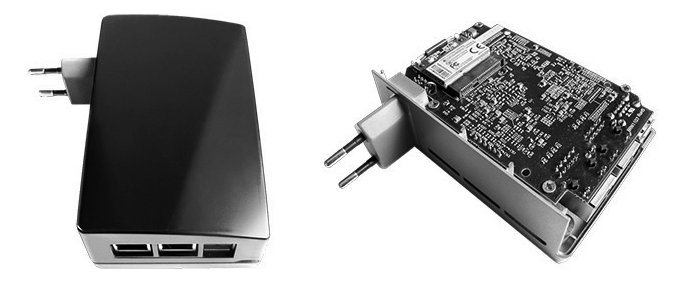
\includegraphics[width=0.3\textwidth]{53_spons_promwad_ip-plug-server_print.jpg}\\[4em]% here too
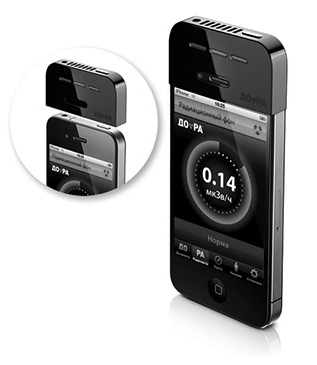
\includegraphics[width=0.3\textwidth]{53_spons_promwad_dora_iphone_enclosure_print.jpg}
\end{center}
\end{wrapfigure}
\begin{itemize}
\item Спроектирован plug-компьютер на базе Linux и С++ "--- аппаратно"=программная
платформа и корпус. Новинка предназначена для решения целого спектра задач в
IP-сетях, а по размерам сопоставима с зарядным устройством для мобильного
телефона.
\item Разработан тонкий клиент AKT-1100 "--- компьютер на базе процессора Marvell Sheeva
(2 ГГц) и ОС Debian Linux 6.0, он переносит процессы обработки данных на
удаленный сервер, использует различные методы защиты информации.
\item Разработан корпус дозиметра"=радиометра <<ДО-РА>> "---  миниатюрного
устройства для измерения радиации (в виде насадки для мобильных телефонов).
Промышленные дизайнеры и конструкторы Promwad разработали стильный корпус
<<ДО-РА>> для iPhone 4 и 4s, он подключается к смартфону через аудиоджек.
\end{itemize}% hackish
~\\[-2.3em]\begin{itemize}% dirty hack to overcome wrapfig problems, don't change, magic involved!
\item Разработан процессорный модуль Automotive Jade на базе ОС Linux и системы
OpenEmbedded для управления, контроля и диагностики оборудования
автотранспорта.
\end{itemize}
Головной центр разработок Promwad размещен в Минске, но его сотрудники видят
результат своей работы в устройствах и программах, которыми пользуются люди по
всему миру.

Ценности компании: непрерывное обучение и внедрение инноваций, открытость к
сотрудничеству и активный отдых (Promwad является титульным спонсором
белорусского кубка приключенческих гонок <<Промвад Тур>>).


